\section{Introduction}

TV archives maintained by national institutions such as the French INA, the Netherlands Institute for Sound \& Vision, or the British Broadcasting Corporation are rapidly growing in size. The need for applications that make these archives searchable has led researchers to devote concerted effort to developing technologies that create indexes.

Indexes that represent the location and identity of people in the archive are indispensable for searching archives. Human nature leads people to be very interested in other people. However, when the content is created or broadcasted, it is not always possible to predict which people will be the most important to find in the future
and biometric models may not yet be available at indexing time
The goal of this task is thus to address the challenge of indexing people in the archive under real-world conditions, \emph{i.e.} when there is no pre-set list of people to index.

Started in 2011, the REPERE challenge aimed at supporting research on multimodal person recognition~\cite{BERNARD--SLAM--2013, KAHN--CBMI--2012}. Its main goal was to answer the two questions \emph{``who speaks when?''} and \emph{``who appears when?''} using any available source of information (including pre-existing biometric models and person names extracted from text overlay and speech transcripts). Thanks to this challenge and the associated multimodal corpus~\cite{GIRAUDEL--LREC--2012}, significant progress was achieved in either supervised or unsupervised multimodal person recognition~\cite{BECHET--INTERSPEECH--2014, BENDRIS--CBMI--2013, BREDIN--ODYSSEY--2014, BREDIN--INTERSPEECH--2013, BREDIN--SLAM--2013, BREDIN--IJMIR--2014, FAVRE--SLAM--2013, GAY--CBMI--2014, POIGNANT--ASLP--2015, POIGNANT--SLAM--2013, POIGNANT--INTERSPEECH--2012, POIGNANT--MTAP--2015, ROUVIER--CBMI--2014}.
After the end of the REPERE challenge in 2014, the  first edition of the ``Multimodal Person Discovery in Broadcast TV'' task was organized in 2015 \cite{POIGNANT--MEDIAEVAL--2015}. This year's task is a follow-up of last year edition.

\subsection{Person discovery in TV broadcast}

Participants are provided with a collection of TV broadcast recordings pre-segmented into shots.
Each shot $s \in \shots$ has to be automatically tagged with the names of people both speaking and appearing at the same time during the shot.

As last year, the list of persons is not provided \emph{a priori}, and person biometric models (neither voice nor face) can not be trained on external data in the primary runs. The only way to identify a person is by finding their name $n \in \hypNames$ in the audio (\emph{e.g.}, using speech transcription -- ASR) or visual (\emph{e.g.}, using optical character recognition -- OCR) streams and associating them to the correct person. This makes the task completely unsupervised (\emph{i.e.} using algorithms not relying on pre-existing labels or biometric models). The main novelty of this year task is that participants may use their contrastive run to try brave new ideas that may rely on any external data, including textual metadata provided with the test set.

Because person names are detected and transcribed automatically, they may contain transcription errors to a certain extent (more on that later in Section~\ref{sec:metric}). In the following, we denote by $\refNames$ the set of all possible person names in the universe, correctly formatted as \texttt{firstname\_lastname} -- while $\hypNames$ is the set of hypothesized names.

\subsection{A system overview}

\section{Overview}

Given the raw TV broadcasts, each shot must be automatically tagged with the name(s) of people who can be both seen as well as heard in the shot along with the confident score. The list of people is not known apriori and their names must be discovered from video text overlay or speech transcripts~\cite{bredin2016mediaeval}. 
%
To this end, a video must be segmented in an unsupervised way into homogeneous segments according to person identity, like  speaker diarization and face diarization, to be combined with the extracted names.
% . Combined with the extracted names,  audio-visual person diarization makes it possible to identify people in videos. % \cite{Gay:Frontiers:2016}.
%

%\begin{figure}[tb]
%\centering
%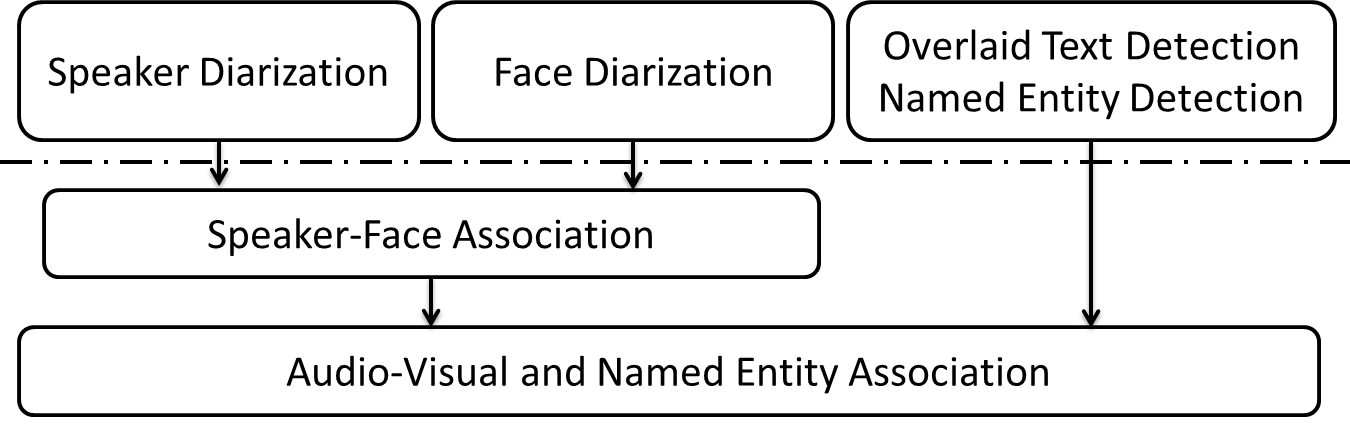
\epsfig{file=diagram.png,width=70mm}
%\vspace*{-3mm}
%\caption{Architecture of our system}
%\vspace*{-3mm}
%\label{fig:pipeline}
%\end{figure}

The overall system is illustrated in Fig.~\ref{fig:pipeline}. It consists of  4 main parts: video optical character recognition (OCR) and named entity recognition (NER), face diariation, speaker diarization, and fusion naming. Each of these parts will be described in the following sections.

\endinput


\endinput
